% Options for packages loaded elsewhere
\PassOptionsToPackage{unicode}{hyperref}
\PassOptionsToPackage{hyphens}{url}
\PassOptionsToPackage{dvipsnames,svgnames,x11names}{xcolor}
%
\documentclass[
  letterpaper,
  DIV=11,
  numbers=noendperiod]{scrartcl}

\usepackage{amsmath,amssymb}
\usepackage{iftex}
\ifPDFTeX
  \usepackage[T1]{fontenc}
  \usepackage[utf8]{inputenc}
  \usepackage{textcomp} % provide euro and other symbols
\else % if luatex or xetex
  \usepackage{unicode-math}
  \defaultfontfeatures{Scale=MatchLowercase}
  \defaultfontfeatures[\rmfamily]{Ligatures=TeX,Scale=1}
\fi
\usepackage{lmodern}
\ifPDFTeX\else  
    % xetex/luatex font selection
\fi
% Use upquote if available, for straight quotes in verbatim environments
\IfFileExists{upquote.sty}{\usepackage{upquote}}{}
\IfFileExists{microtype.sty}{% use microtype if available
  \usepackage[]{microtype}
  \UseMicrotypeSet[protrusion]{basicmath} % disable protrusion for tt fonts
}{}
\makeatletter
\@ifundefined{KOMAClassName}{% if non-KOMA class
  \IfFileExists{parskip.sty}{%
    \usepackage{parskip}
  }{% else
    \setlength{\parindent}{0pt}
    \setlength{\parskip}{6pt plus 2pt minus 1pt}}
}{% if KOMA class
  \KOMAoptions{parskip=half}}
\makeatother
\usepackage{xcolor}
\setlength{\emergencystretch}{3em} % prevent overfull lines
\setcounter{secnumdepth}{-\maxdimen} % remove section numbering
% Make \paragraph and \subparagraph free-standing
\ifx\paragraph\undefined\else
  \let\oldparagraph\paragraph
  \renewcommand{\paragraph}[1]{\oldparagraph{#1}\mbox{}}
\fi
\ifx\subparagraph\undefined\else
  \let\oldsubparagraph\subparagraph
  \renewcommand{\subparagraph}[1]{\oldsubparagraph{#1}\mbox{}}
\fi


\providecommand{\tightlist}{%
  \setlength{\itemsep}{0pt}\setlength{\parskip}{0pt}}\usepackage{longtable,booktabs,array}
\usepackage{calc} % for calculating minipage widths
% Correct order of tables after \paragraph or \subparagraph
\usepackage{etoolbox}
\makeatletter
\patchcmd\longtable{\par}{\if@noskipsec\mbox{}\fi\par}{}{}
\makeatother
% Allow footnotes in longtable head/foot
\IfFileExists{footnotehyper.sty}{\usepackage{footnotehyper}}{\usepackage{footnote}}
\makesavenoteenv{longtable}
\usepackage{graphicx}
\makeatletter
\def\maxwidth{\ifdim\Gin@nat@width>\linewidth\linewidth\else\Gin@nat@width\fi}
\def\maxheight{\ifdim\Gin@nat@height>\textheight\textheight\else\Gin@nat@height\fi}
\makeatother
% Scale images if necessary, so that they will not overflow the page
% margins by default, and it is still possible to overwrite the defaults
% using explicit options in \includegraphics[width, height, ...]{}
\setkeys{Gin}{width=\maxwidth,height=\maxheight,keepaspectratio}
% Set default figure placement to htbp
\makeatletter
\def\fps@figure{htbp}
\makeatother

\KOMAoption{captions}{tableheading}
\makeatletter
\@ifpackageloaded{caption}{}{\usepackage{caption}}
\AtBeginDocument{%
\ifdefined\contentsname
  \renewcommand*\contentsname{Table of contents}
\else
  \newcommand\contentsname{Table of contents}
\fi
\ifdefined\listfigurename
  \renewcommand*\listfigurename{List of Figures}
\else
  \newcommand\listfigurename{List of Figures}
\fi
\ifdefined\listtablename
  \renewcommand*\listtablename{List of Tables}
\else
  \newcommand\listtablename{List of Tables}
\fi
\ifdefined\figurename
  \renewcommand*\figurename{Figure}
\else
  \newcommand\figurename{Figure}
\fi
\ifdefined\tablename
  \renewcommand*\tablename{Table}
\else
  \newcommand\tablename{Table}
\fi
}
\@ifpackageloaded{float}{}{\usepackage{float}}
\floatstyle{ruled}
\@ifundefined{c@chapter}{\newfloat{codelisting}{h}{lop}}{\newfloat{codelisting}{h}{lop}[chapter]}
\floatname{codelisting}{Listing}
\newcommand*\listoflistings{\listof{codelisting}{List of Listings}}
\makeatother
\makeatletter
\makeatother
\makeatletter
\@ifpackageloaded{caption}{}{\usepackage{caption}}
\@ifpackageloaded{subcaption}{}{\usepackage{subcaption}}
\makeatother
\ifLuaTeX
  \usepackage{selnolig}  % disable illegal ligatures
\fi
\usepackage{bookmark}

\IfFileExists{xurl.sty}{\usepackage{xurl}}{} % add URL line breaks if available
\urlstyle{same} % disable monospaced font for URLs
\hypersetup{
  pdftitle={Projeto fantasma},
  colorlinks=true,
  linkcolor={blue},
  filecolor={Maroon},
  citecolor={Blue},
  urlcolor={Blue},
  pdfcreator={LaTeX via pandoc}}

\title{Projeto fantasma}
\author{}
\date{}

\begin{document}
\maketitle

\section{Introdução}\label{introduuxe7uxe3o}

Este projeto tem como objetivo A fim de atender a demanda do cliente,
foi feita uma análise estatistica descritiva acerca dos atletas que
participaram das olimpiadas dos anos de 2000 até 2016.

O banco de dados foi disponibilizado pelo cliente. Foi observado nome,
sexo, idade, país, peso, altura, esporte, modalidade e medalha adquirida
de 38366 atletas diferentes.

A manipulação e análise dos dados além da confecção das figuras foram
feitas com auxilio do software estatístico R versão 4.3.3.

\section{Referencial Teórico}\label{referencial-teuxf3rico}

\section{Análises}\label{anuxe1lises}

\subsubsection{1. Top 5 países com maior número de mulheres
medalistas}\label{top-5-pauxedses-com-maior-nuxfamero-de-mulheres-medalistas}

Está análise tem o intuito de identificar quais são os países com maior
quantidade de mulheres medalhistas. Para isso foram utilizadas as
variáveis sexo e medalhas, a primeira sendo qualitativa nominal e a
sugunda sendo qualitativa ordinal.

\paragraph{Figura 1: gráfico de colunas do número de mulheres
medalistas}\label{figura-1-gruxe1fico-de-colunas-do-nuxfamero-de-mulheres-medalistas}

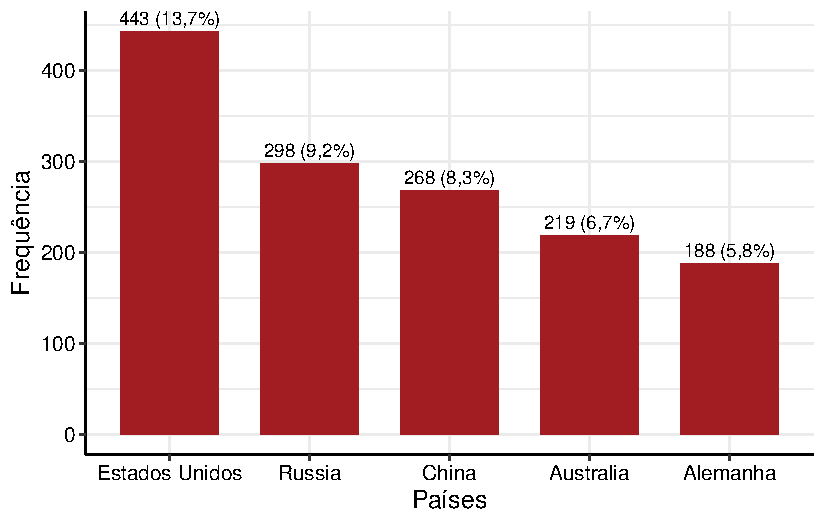
\includegraphics{Relatorio-projeto-fantasma_files/figure-pdf/unnamed-chunk-2-1.pdf}

Como pode ser observado na figura 1, o ranque é formado por Estados
unidos, Rússia, China, Australia e Alemanha respectivamente. Os Estados
Unidos ocupa o primeiro lugar do ranque com mais de 100 medalhas de
diferença da Rússia. Juntos esses 5 países sozinhos tem 43,7\% das
mulheres medalistas.

\subsubsection{2. IMC por esportes}\label{imc-por-esportes}

Essa análise tem como objetivo entender o comportamento do IMC nos
esportes selecionados. Para tal, foram utilizadas as variáveis esporte e
IMC,respectivamente qualitativa nominal e quantitativa continua. A
variável IMC foi obtida dividindo o peso do atleta pela altura ao
quadrado.O valor do índice de massa corporal(IMC) é um importante
indicador da saúde de uma pessoa. o número representa o quanto a pessoa
tem de massa muscular + massa de gordura + massa óssea.

\paragraph{Figura 2: Boxplot do IMC pelo
Esporte}\label{figura-2-boxplot-do-imc-pelo-esporte}

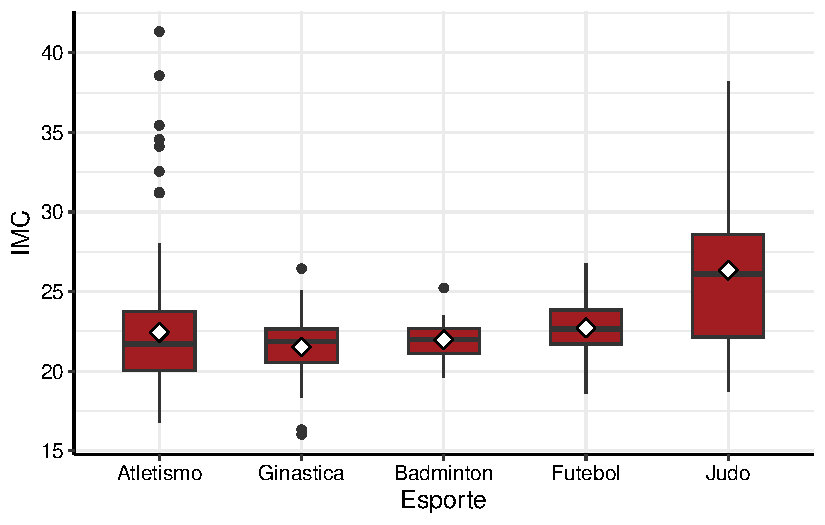
\includegraphics{Relatorio-projeto-fantasma_files/figure-pdf/unnamed-chunk-3-1.pdf}

\paragraph{Figura 3}\label{figura-3}

\begin{verbatim}
NA
\end{verbatim}

Pode se observar que o IMC segue um comportamento diferente para cada
esporte. No judô há diversas categorias para pessoas com pesos
diferentes e é um esporte que exige maior massa muscular, o que explica
a maior dispersão dos dados (Desvio padrão=6.24) e uma média
elevada(26.78) se comparada com as dos outros esportes. A medida de
centralidade média no Badminton, na Ginastica, no futebol e no Atletismo
são semelhantes: 22.17, 20.76, 22.72 e 22.12 respectivamente, entretanto
cada um tem uma configuração única. No atletismo há uma assimetria
positiva, na ginastica há uma assimetria negativa e no badminton e no
futebol a distribuição é simetrica e centralizada(desvio padrão=1.61).
Em geral, quanto mais um esporte ou modalidade exige massa muscular,
maior o IMC.

\subsubsection{3. Top 3 medalhistas
gerais}\label{top-3-medalhistas-gerais}

Esta análise tem como objetivo observar quais são os 3 maiores
medalhistas e verificar se há relação entre o medalhista e o tipo de
medalha conquistada. Os três atletas que conquistaram mais medalhas
nessas 5 edições dos jogos olímpicos foram: Michael Fred Phelps com 28
medalhas, Natalie Anne Coughlin e Ryan Steven Lochte ambos com 12
medalhas. Os três são estadunidenses e tem como esporte a natação.

\paragraph{Figura 4: Gráfico de colunas da quantidade de medalhas pelo
tipo da
medalha}\label{figura-4-gruxe1fico-de-colunas-da-quantidade-de-medalhas-pelo-tipo-da-medalha}

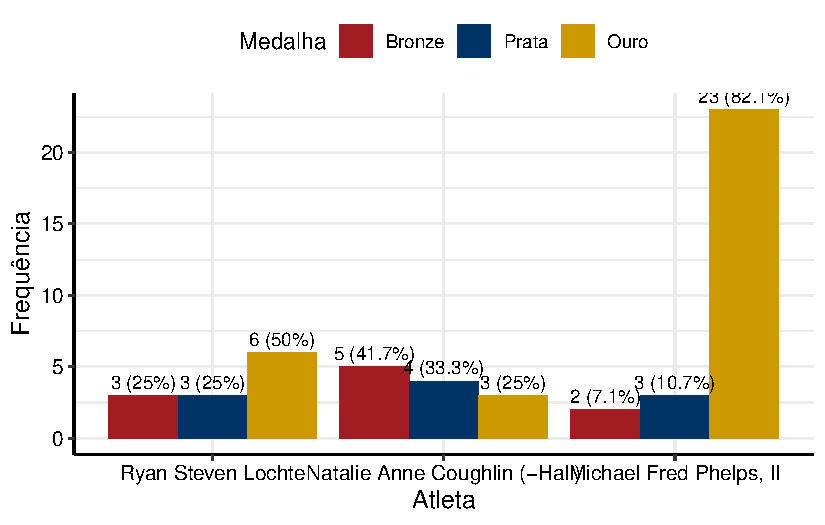
\includegraphics{Relatorio-projeto-fantasma_files/figure-pdf/unnamed-chunk-5-1.pdf}

Observa-se pelo gráfico a relação entre o atleta e o tipo de medalha.
Conforme o valor da medalha aumentou, Natalie conquistou menos medalhas,
enquanto para Michael e Ryan o comportamento foi o contrário. Também é
possivel observar que a grande maioria das medalhas que Michael Fred
Phelps conquistou foram medalhas de ouro.

\subsubsection{4. Relação peso x
altura}\label{relauxe7uxe3o-peso-x-altura}

Esta análise tem o intuito de compreender a relação entre o peso e a
altura dos atletas. Para isso, foi utilizado as variáveis peso(Kg) e
altura(m), ambas são quantitativas continuas. O comportamento conjunto
das variáveis está ilustrado pelo gráfico de dispersão a seguir:

\paragraph{Figura 5: Gráfico de dispersão do peso pela altura do
atleta}\label{figura-5-gruxe1fico-de-dispersuxe3o-do-peso-pela-altura-do-atleta}

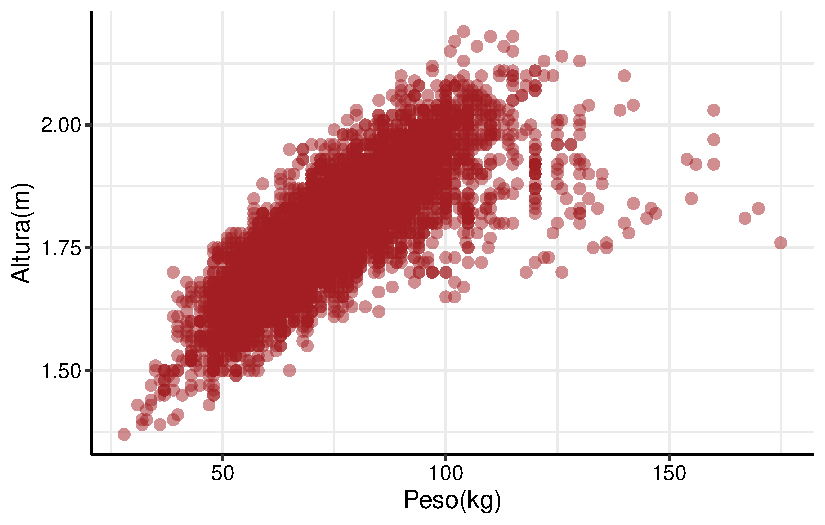
\includegraphics{Relatorio-projeto-fantasma_files/figure-pdf/unnamed-chunk-6-1.pdf}

\paragraph{Quadro 2: Medidas resumo das variáveis peso e altura do
atleta}\label{quadro-2-medidas-resumo-das-variuxe1veis-peso-e-altura-do-atleta}

\begin{verbatim}
         Medida Peso(Kg) Altura(m)
1         Média    74.14      1.78
2 Desvio Padrão    16.25      0.12
3     Variância   264.05      0.01
4        Mínimo    28.00      1.37
5    1° quartil    62.99      1.70
6       Mediana    71.99      1.78
7    3° quartil    83.99      1.86
8        Máximo   174.97      2.19
\end{verbatim}

print_quadro_resumo <- function(data, var_name, title="Medidas resumo
da(o) [nome da variável]", label="quad:quadro_resumo1") {
  var_name <- substitute(var_name)
  data <- data %>%
    summarize(`Média` = round(mean(!!sym(var_name),na.rm = T),2),
              `Desvio Padrão` = round(sd(!!sym(var_name),na.rm = T),2),
              `Variância` = round(var(!!sym(var_name),na.rm = T),2),
              `Mínimo` = round(min(!!sym(var_name),na.rm = T),2),
              `1º Quartil` = round(quantile(!!sym(var_name), probs =
                                              .25,na.rm = TRUE),2),
              `Mediana` = round(quantile(!!sym(var_name), probs = .5,na.rm = TRUE)
                                ,2),
              `3º Quartil` = round(quantile(!!sym(var_name), probs =
                                              .75,na.rm = TRUE),2),
              `Máximo` = round(max(!!sym(var_name),na.rm = T),2)) %>%
    t() %>%
    as.data.frame() %>%
    rownames_to_column()
  latex <- str_c("\\begin{quadro}[H]
\t\\caption{", title, "}
\t\\centering
\t\\begin{adjustbox}{max width=\\textwidth}
\t\\begin{tabular}{", sep="")
  col_count <- ncol(data)
  row_count <- nrow(data)
  latex <- str_c(latex, "| l |\n", sep=" ")
  for (i in seq(2, col_count))
  {
    numCount <- data[i, -c(1)] %>%
      as.numeric() %>%
      {floor(log10(.)) + 1} %>%
      max()
    latex <- str_c(latex, "\t\t\tS[table-format = ", numCount ,".2]\n
", sep="")
  }
  latex <- str_c(latex, "\t\t\t|}\n\t\\toprule\n\t\t", sep="")
  if (col_count > 2)
  {
    for (i in seq(1,col_count))
    {
      if (i == 1)
        latex <- str_c(latex, "\\textbf{Estatística}", sep="")
      else
        latex <- str_c(latex, " \\textbf{", data[1, i], "}", sep="")
      if (i < col_count)
        latex <- str_c(latex, "&", sep=" ")
      else
        latex <- str_c(latex, "\\\\\n", sep=" ")
    }
  }
  else
  {
    latex <- str_c(latex, "\\textbf{Estatística} & \\textbf{Valor}
\\\\\n", sep="")
  }
  latex <- str_c(latex, "\t\t\\midrule\n", sep="")
  if (col_count > 2)
    starting_number <- 2
  else
    starting_number <- 1
  for (i in seq(starting_number, row_count))
  {
    latex <- str_c(latex, "\t\t", str_flatten(t(data[i,]), collapse =
                                                " & "), " \\\\\n")
  }
  latex <- str_c(latex, "\t\\bottomrule
  \t\\end{tabular}
\t\\label{", label, "}
\t\\end{adjustbox}
\\end{quadro}", sep="")
  writeLines(latex)
}
PMD %>% print_quadro_resumo(var_name = "Peso(kg)")

Os atletas tem, em geral, peso entre 63 e 84 quilos e altura entre 1.70
e 1.86 metros, além disso o peso dos atletas varia mais que a
altura(coeficiente de variação 0.21 e 0.06 respectivamente) . O
coeficiente de Pearson, que mostra a força e o sentido da associação de
duas variaveis quantitativas e varia de -1 a 1, assumiu o valor 0.79, ou
seja, observa se pelo gráfico e pelo coeficiente uma relação forte e
positiva entre as variáveis, conforme a altura aumenta o peso tende a
aumentar.

\section{Conclusões}\label{conclusuxf5es}



\end{document}
